\documentclass[10pt,a4paper,oneside]{99_fhnwreport}
% \documentclass[10pt,a4paper,oneside]{article}

%%%%%%%%%%%%%%%%%%%%%%%%%%%%%%%%%%%%%%%%%%%%%%%%%%%%%%%%%%%%%%%%%%%%%%%%%%%%%%%%
% basic font and language packages
%%%%%%%%%%%%%%%%%%%%%%%%%%%%%%%%%%%%%%%%%%%%%%%%%%%%%%%%%%%%%%%%%%%%%%%%%%%%%%%%
% \usepackage[left=35mm,right=35mm,top=35mm,bottom=30mm]{geometry}
\usepackage[T1]{fontenc} % font encoding
\usepackage{lmodern} % font latin modern
\usepackage[utf8]{inputenc} % input encoding
\usepackage[ngerman]{babel} % english and german word spelling
\usepackage[babel, german=swiss]{csquotes} % german cites
%\usepackage[babel, english=british]{csquotes} % english cites

%%%%%%%%%%%%%%%%%%%%%%%%%%%%%%%%%%%%%%%%%%%%%%%%%%%%%%%%%%%%%%%%%%%%%%%%%%%%%%%%
% style packages
%%%%%%%%%%%%%%%%%%%%%%%%%%%%%%%%%%%%%%%%%%%%%%%%%%%%%%%%%%%%%%%%%%%%%%%%%%%%%%%%
\usepackage{hyperref} % use hyperlinks in table of contents
\hypersetup{colorlinks=true,urlcolor=blue,linkcolor=black} % define hyperlink colors
\usepackage{verbatim} % don't interpret latex symbols (source code)
\usepackage{enumerate} % numbered items
\usepackage{graphicx} % use figures
\usepackage{subfigure} % more than one figure in the same place
\usepackage{booktabs} % create tables
\usepackage{multirow} % create tables
\usepackage{cite} % citations
\usepackage{pdflscape} % allow landscape sites in pdf documents
\usepackage{pdfpages} % include pdf files

%%%%%%%%%%%%%%%%%%%%%%%%%%%%%%%%%%%%%%%%%%%%%%%%%%%%%%%%%%%%%%%%%%%%%%%%%%%%%%%%
% mathematical packages
%%%%%%%%%%%%%%%%%%%%%%%%%%%%%%%%%%%%%%%%%%%%%%%%%%%%%%%%%%%%%%%%%%%%%%%%%%%%%%%%
\usepackage{amsmath} % formula
\usepackage{amsfonts} % formula
\usepackage{amssymb} % formula
\usepackage{amsthm} % formula
\usepackage{listings} % source code formatting

%%%%%%%%%%%%%%%%%%%%%%%%%%%%%%%%%%%%%%%%%%%%%%%%%%%%%%%%%%%%%%%%%%%%%%%%%%%%%%%%
% optional parameters
%%%%%%%%%%%%%%%%%%%%%%%%%%%%%%%%%%%%%%%%%%%%%%%%%%%%%%%%%%%%%%%%%%%%%%%%%%%%%%%%
\bibliographystyle{IEEEtran}
\graphicspath{{./graphics/}{./appendix/}}

% source code parameters
\lstset{numbers=left, numberstyle=\tiny, numbersep=6pt}
\lstset{captionpos=b, tabsize=4, basicstyle=\small, xleftmargin=0mm, xrightmargin=0mm}

%%%%%%%%%%%%%%%%%%%%%%%%%%%%%%%%%%%%%%%%%%%%%%%%%%%%%%%%%%%%%%%%%%%%%%%%%%%%%%%%
% debugging parameters
%%%%%%%%%%%%%%%%%%%%%%%%%%%%%%%%%%%%%%%%%%%%%%%%%%%%%%%%%%%%%%%%%%%%%%%%%%%%%%%%
%\usepackage{todonotes}
%\overfullrule=1em

%%%%%%%%%%%%%%%%%%%%%%%%%%%%%%%%%%%%%%%%%%%%%%%%%%%%%%%%%%%%%%%%%%%%%%%%%%%%%%%%
% document settings
%%%%%%%%%%%%%%%%%%%%%%%%%%%%%%%%%%%%%%%%%%%%%%%%%%%%%%%%%%%%%%%%%%%%%%%%%%%%%%%%
%\title{Title\\\large Undertitle}
\title{
	\textsc{\LARGE{Organisatorisches-Pflichtenheft}}\\[10mm]
	\textsc{\LARGE{Dojo - Mehr als nur ein Museumsguide}}
}

\author{}

\date{\today}

%%%%%%%%%%%%%%%%%%%%%%%%%%%%%%%%%%%%%%%%%%%%%%%%%%%%%%%%%%%%%%%%%%%%%%%%%%%%%%%
% pictures
%\begin{figure}[htb]
%\includegraphics[width=\textwith]{image1.png}
%\figcaption{image1} % picture caption
%\label{fig:image1}
%\end{figure}
%
%(Abb. \ref{fig:image1})
%%%%%%%%%%%%%%%%%%%%%%%%%%%%%%%%%%%%%%%%%%%%%%%%%%%%%%%%%%%%%%%%%%%%%%%%%%%%%%%

%%%%%%%%%%%%%%%%%%%%%%%%%%%%%%%%%%%%%%%%%%%%%%%%%%%%%%%%%%%%%%%%%%%%%%%%%%%%%%%
% equation
%\begin{equation}
%X_{1,2} = \frac{-b \pm \sqrt{b^{2}-4ac}}{2a}
%\label{eq:equation1}
%\end{equation}
%%%%%%%%%%%%%%%%%%%%%%%%%%%%%%%%%%%%%%%%%%%%%%%%%%%%%%%%%%%%%%%%%%%%%%%%%%%%%%%

%%%%%%%%%%%%%%%%%%%%%%%%%%%%%%%%%%%%%%%%%%%%%%%%%%%%%%%%%%%%%%%%%%%%%%%%%%%%%%%
% table
%\begin{table}[tb]
%\centering
%\begin{tabular}
%
%\end{tabular}
%\caption{Table 1}
%\label{tab:table1}
%\end{table}
%%%%%%%%%%%%%%%%%%%%%%%%%%%%%%%%%%%%%%%%%%%%%%%%%%%%%%%%%%%%%%%%%%%%%%%%%%%%%%%

%%%%%%%%%%%%%%%%%%%%%%%%%%%%%%%%%%%%%%%%%%%%%%%%%%%%%%%%%%%%%%%%%%%%%%%%%%%%%%%
% citation
%\cite{BUCH1}
%%%%%%%%%%%%%%%%%%%%%%%%%%%%%%%%%%%%%%%%%%%%%%%%%%%%%%%%%%%%%%%%%%%%%%%%%%%%%%%

%%%%%%%%%%%%%%%%%%%%%%%%%%%%%%%%%%%%%%%%%%%%%%%%%%%%%%%%%%%%%%%%%%%%%%%%%%%%%%%
% source code
%\begin{lstlisting}[frame=tb,caption={Application.java}, label=lst:code, language=java]
%your source code
%\end{lstlisting}
% or
%\lstinputlisting[frame=tb,caption={Caption 1}, label=lst:code1, language=c]{path/file.src}
%
%%%%%%%%%%%%%%%%%%%%%%%%%%%%%%%%%%%%%%%%%%%%%%%%%%%%%%%%%%%%%%%%%%%%%%%%%%%%%%%

\begin{document}
%%%%%%%%%%%%%%%%%%%%%%%%%%%%%%%%%%%%%%%%%%%%%%%%%%%%%%%%%%%%%%%%%%%%%%%%%%%%%%%%
% title page
%%%%%%%%%%%%%%%%%%%%%%%%%%%%%%%%%%%%%%%%%%%%%%%%%%%%%%%%%%%%%%%%%%%%%%%%%%%%%%%%
\pagenumbering{gobble}
\maketitle

\noindent % einzug
\rule{\linewidth}{0.5mm}

\textsc{
\begin{tabbing}
\hspace{40mm}	\= \hspace{15mm} \=\kill
Auftraggeber	\> Jana Kalbermatter und Hans Gysin \\[5mm]
Fachcoaches	\> Matthias Meier und Pascal Schleuniger\\[5mm]
Projektleiter	\> Dominik Hiltbrunner\\
Team		\> Alexander Stutz, Emerson Lattmann, \\
		\> Pius Ochs, Tobias Klenke und Roman Sonder\\[5mm]
Studiengang	\> Elektro- und Informationstechnik \\[5mm]
\end{tabbing}
}

\clearpage
\color{black}

%%%%%%%%%%%%%%%%%%%%%%%%%%%%%%%%%%%%%%%%%%%%%%%%%%%%%%%%%%%%%%%%%%%%%%%%%%%%%%%%
% table of contents
%%%%%%%%%%%%%%%%%%%%%%%%%%%%%%%%%%%%%%%%%%%%%%%%%%%%%%%%%%%%%%%%%%%%%%%%%%%%%%%%
\pagenumbering{roman}
\setcounter{page}{1}
\tableofcontents
\clearpage

%%%%%%%%%%%%%%%%%%%%%%%%%%%%%%%%%%%%%%%%%%%%%%%%%%%%%%%%%%%%%%%%%%%%%%%%%%%%%%%%
% Einleitung
%%%%%%%%%%%%%%%%%%%%%%%%%%%%%%%%%%%%%%%%%%%%%%%%%%%%%%%%%%%%%%%%%%%%%%%%%%%%%%%%
\pagenumbering{arabic}
\setcounter{page}{1}
\section{Einleitung}\label{sec:einleitung}
Ziel dieses Projektes ist es, ein Museumsführer namens Dojo zu realisieren.
Dojo wurde funktionell und gestalterisch von Jana Kalbermatter entwickelt.
Somit fehlt es dem Dojo-Gehäuse an Elektronik. Dies soll in diesem Projekt realisiert werden.
Dojo ist ein moderner Museumführer, der ohne Kopfhörer auskommt. Mittels Knochenschallgeber soll der Benutzer die Informationen über die jeweiligen Kunstobjekte erhalten.
Das stabförmige Gerät informiert via Körperschallübertragung über alle Kunstobjekte in dessen Nähe man sich aufhält. Man muss lediglich das Ende des Stabes hinter das Ohr halten und hört die «Geisterstimme» mit den Ausführungen zum Kunstobjekt.

%%%%%%%%%%%%%%%%%%%%%%%%%%%%%%%%%%%%%%%%%%%%%%%%%%%%%%%%%%%%%%%%%%%%%%%%%%%%%%%%
% Projektorganisation
%%%%%%%%%%%%%%%%%%%%%%%%%%%%%%%%%%%%%%%%%%%%%%%%%%%%%%%%%%%%%%%%%%%%%%%%%%%%%%%%
\section{Projektorganisation}\label{sec:projektorganisation}

Die Studierenden werden im Projekt4 (pro4E) für den Studiengang Elektro- und Informationstechnik von fünf Dozenten der Fachhochschule Nordwestschweiz (FHNW) unterstützt. Pascal Buchschacher informiert über das Projektmanagement und Roswitha Dubach vermittelt den Studenten die richtige Kommunikation innerhalb des Teams. Ansprechpartner für Fragen technischer Natur sind Pascal Schleuniger, Martin Meier und Hans Gysin, welcher auch als interner Auftraggeber agiert.
Externe und eigentliche Auftraggeberin ist Jana Kalbermatter, eine Absolventin der HGK.

%%%%%%%%%%%%%%%%%%%%%%%%%%%%%%%%%%%%%%%%%%%%%%%%%%%%%%%%%%%%%%%%%%%%%%%%%%%%%%%%
\subsection{Projektteam}\label{subsec:projektteam}
%%%%%%%%%%%%%%%%%%%%%%%%%%%%%%%%%%%%%%%%%%%%%%%%%%%%%%%%%%%%%%%%%%%%%%%%%%%%%%%
Das Team 3 des Projekts 4 setzt sich aus sechs Studenten zusammen. Dominik Hiltbrunner ist der Projektleiter und verantwortlich für die Arbeitsverteilung und die Kommunikation mit den Auftraggebern sowie den Fachdozenten. Unterstützt wird dieser vom stellvertretenden Projektleiter Tobias Klenke. Die übrigen Mitglieder sind Alexander Stutz, Roman Sonder, Pius Ochs und Emerson Lattmann. 
\newpage
%%%%%%%%%%%%%%%%%%%%%%%%%%%%%%%%%%%%%%%%%%%%%%%%%%%%%%%%%%%%%%%%%%%%%%%%%%%%%%%
%Organigramm
%%%%%%%%%%%%%%%%%%%%%%%%%%%%%%%%%%%%%%%%%%%%%%%%%%%%%%%%%%%%%%%%%%%%%%%%%%%%%%%%

\begin{landscape}
\subsection{Organigramm}\label{subsec:organigramm}


\begin{figure}[htbp]
	\centering
	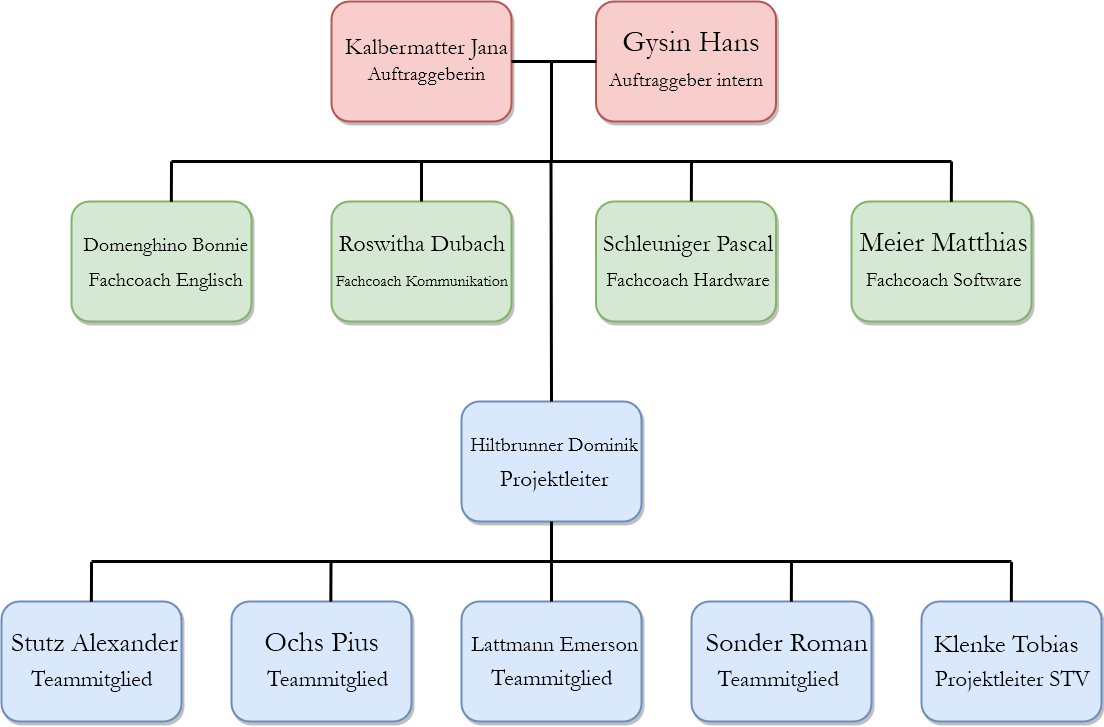
\includegraphics[scale=0.40]{pro4E_Struktur.png}
	\caption{Organigramm}
\end{figure}

%%%%%%%%%%%%%%%%%%%%%%%%%%%%%%%%%%%%%%%%%%%%%%%%%%%%%%%%%%%%%%%%%%%%%%%%%%%%%%%%
% Projektplanung
%%%%%%%%%%%%%%%%%%%%%%%%%%%%%%%%%%%%%%%%%%%%%%%%%%%%%%%%%%%%%%%%%%%%%%%%%%%%%%%%
\section{Projektplanung}\label{sec:projektplanung}
Die Planung des Projektes wird in den folgenden zwei Tabellen dargestellt.
In der Projektplanung ist ersichtlich, welches Teammitglied für welche Aufgaben Verantwortlich ist und wie viele Ressourcen für das jeweilige Arbeitspaket geplant sind. Ausserdem ist ersichtlich, zu welchem Zeitpunkt eine Arbeit erledigt sein sollte.

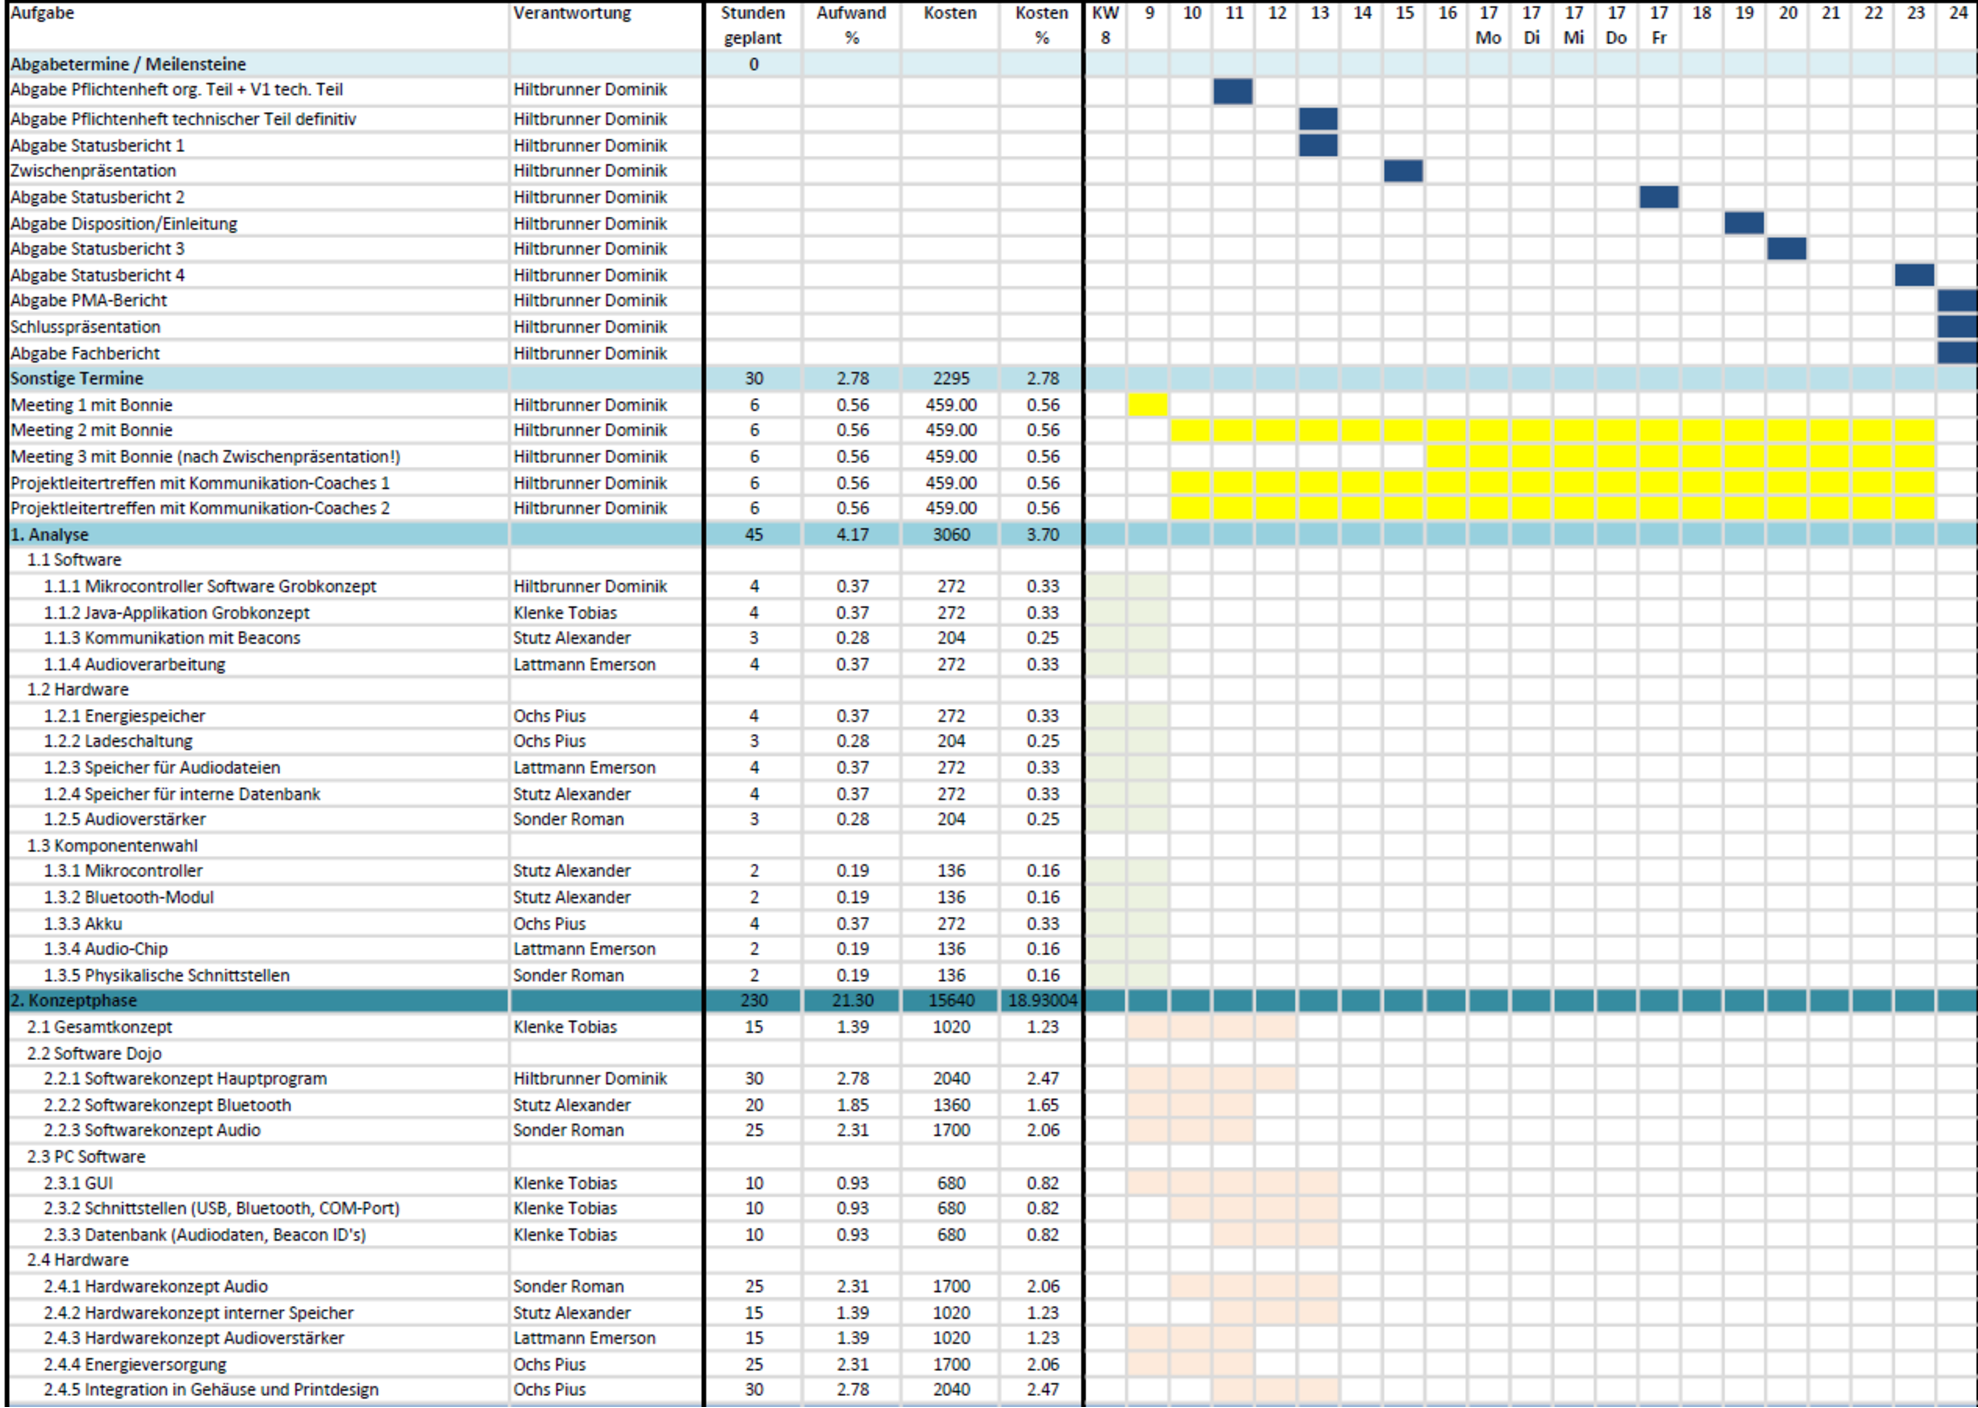
\includegraphics[height=\dimexpr\textheight-4\baselineskip\relax,page=1]{projektplan_1.pdf}
\newpage

\hspace*{-0.6cm}
\vspace*{2cm}
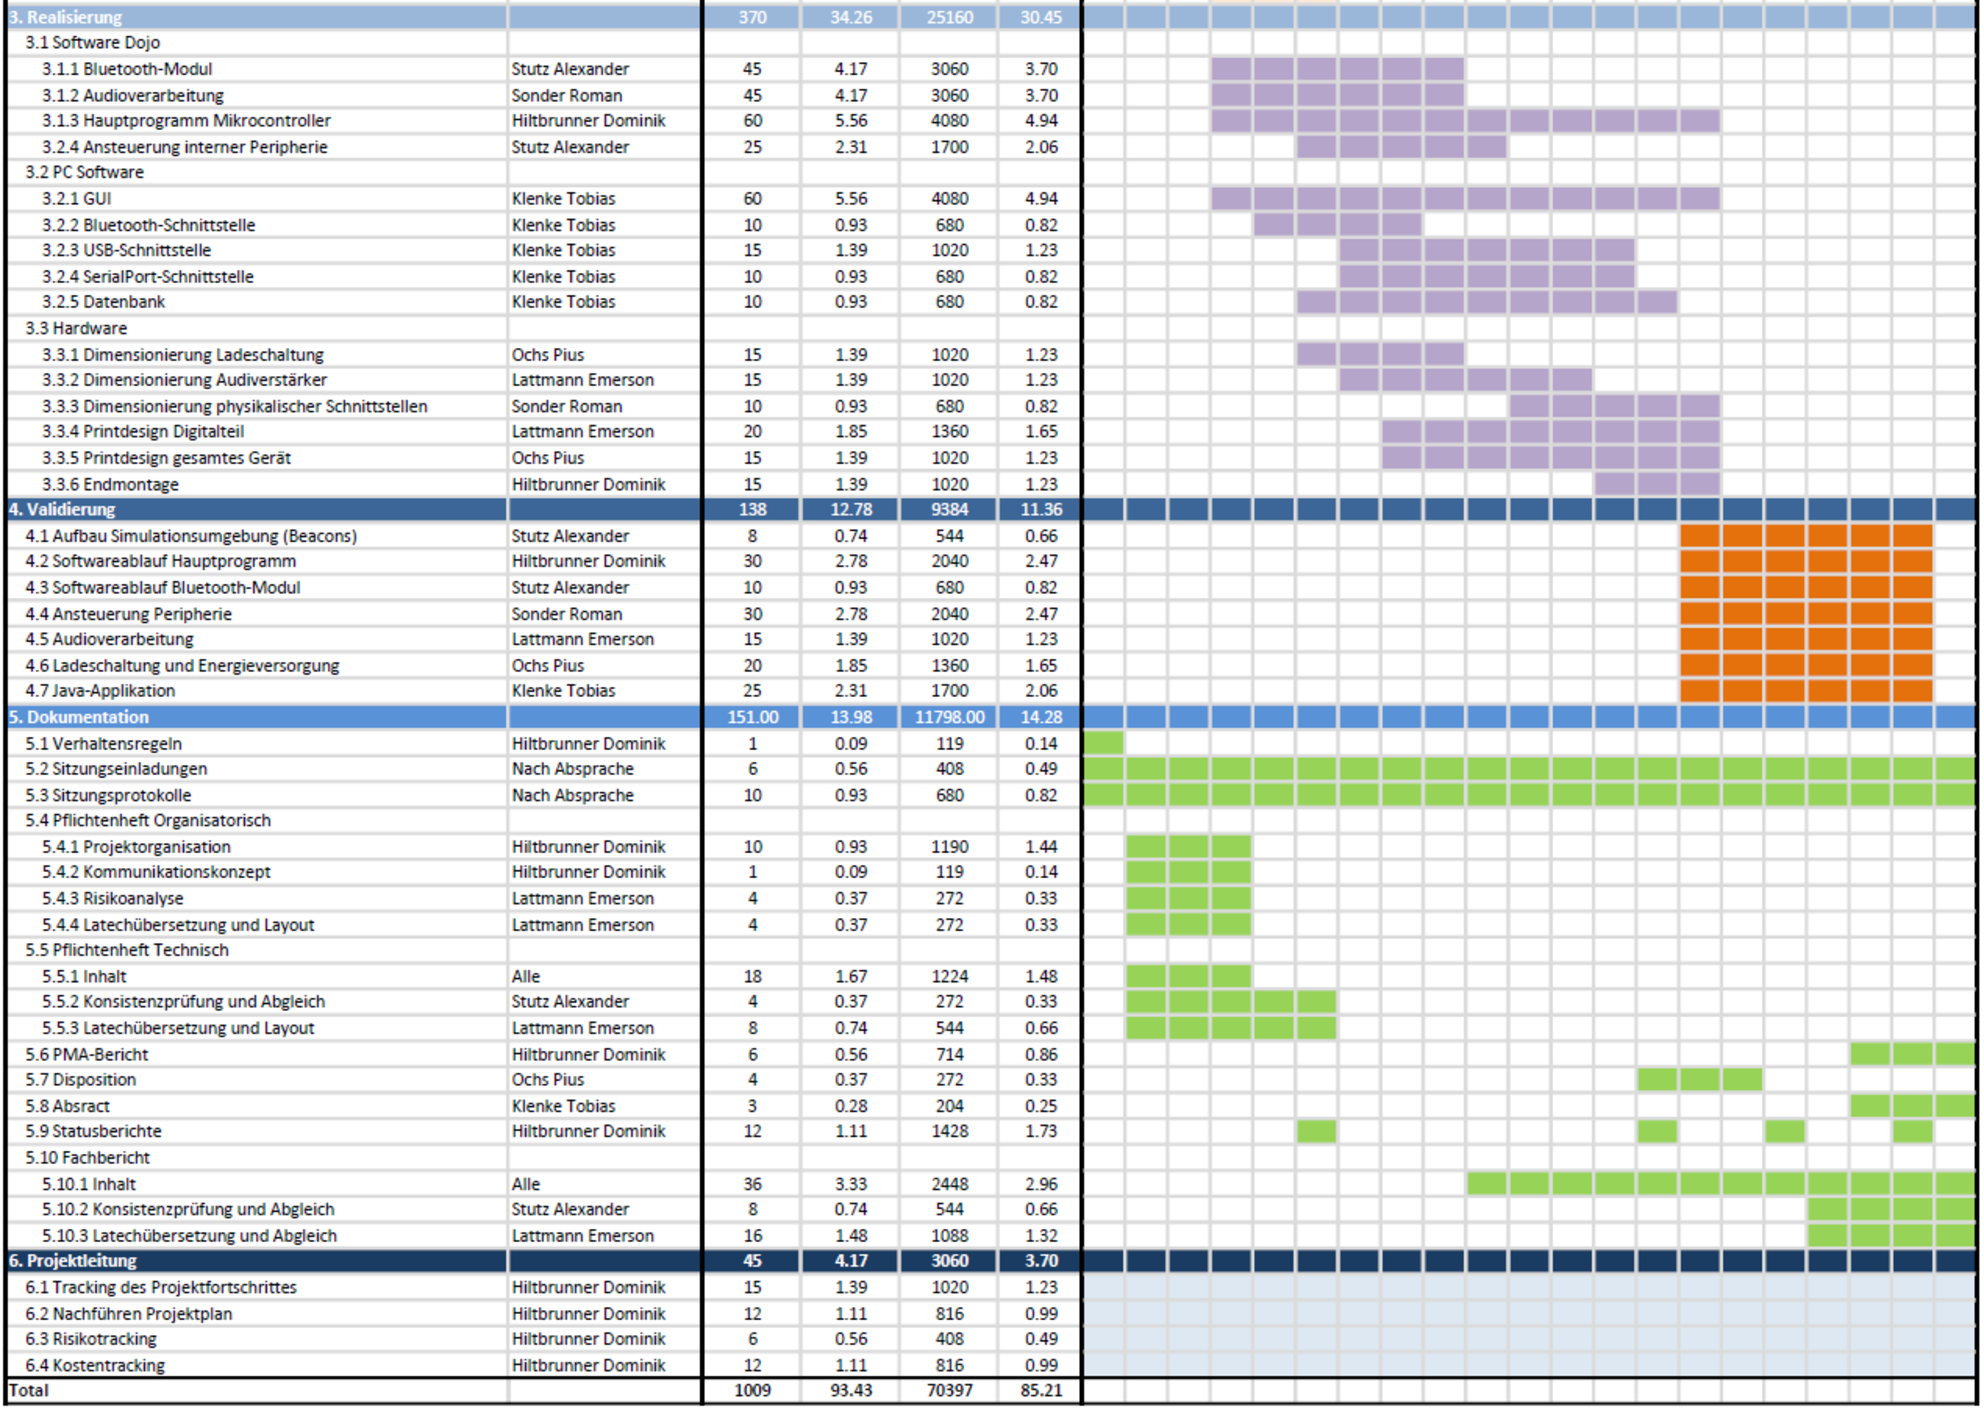
\includegraphics[height=\dimexpr\textheight-4\baselineskip\relax,page=1]{projektplan_2.pdf}
\end{landscape}
\newpage

%%%%%%%%%%%%%%%%%%%%%%%%%%%%%%%%%%%%%%%%%%%%%%%%%%%%%%%%%%%%%%%%%%%%%%%%%%%%%%%%
% Projektbudget
%%%%%%%%%%%%%%%%%%%%%%%%%%%%%%%%%%%%%%%%%%%%%%%%%%%%%%%%%%%%%%%%%%%%%%%%%%%%%%%%
\section{Projektbudget}\label{sec:projektbudget}
In der folgenden Tabelle  werden die Kosten für das Projekt aufgelistet und in verschiedene Bereiche aufgeteilt. Die zwei Hauptbereiche sind der Personalaufwand und der Materialaufwand, welche in weitere kleinere Bereiche aufgeteilt werden.

\noindent
Die detaillierten Angaben zu den Personalkosten können dem Projektplan entnommen werden. Es gelten folgende Stundenansätze:

\begin{tabbing}
\hspace{80mm}			\= 	\hspace{10mm} 	\kill
\textbf{Funktion}		\> \textbf{Stundenansatz in CHF / h} \\
\> \\
Projektleiter 			\>	129 	\\
Wissenschaftlicher Mitarbeiter 	\> 	68	\\
\end{tabbing}

\begin{figure}[htbp]
	\centering
	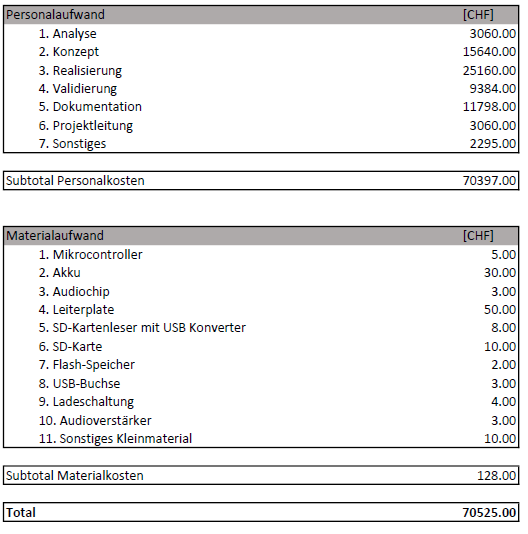
\includegraphics[width=13.5cm]{Projektbudget.png}
\end{figure}


\newpage

%%%%%%%%%%%%%%%%%%%%%%%%%%%%%%%%%%%%%%%%%%%%%%%%%%%%%%%%%%%%%%%%%%%%%%%%%%%%%%%%
% Kommunikationskonzept
%%%%%%%%%%%%%%%%%%%%%%%%%%%%%%%%%%%%%%%%%%%%%%%%%%%%%%%%%%%%%%%%%%%%%%%%%%%%%%%%
\section{Kommunikationskonzept \label{sec:kommunikationskonzept}}

\begin{figure}[htbp]
	\centering
	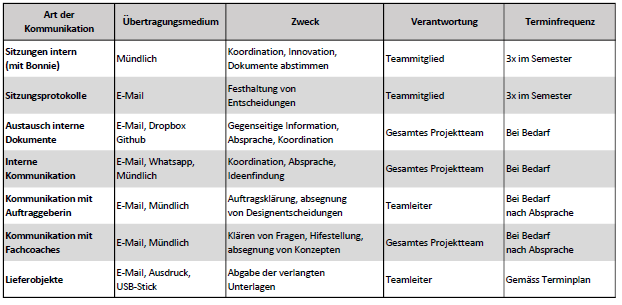
\includegraphics[width=\textwidth]{Kommunikationskonzept.png}
	
\end{figure}

%%%%%%%%%%%%%%%%%%%%%%%%%%%%%%%%%%%%%%%%%%%%%%%%%%%%%%%%%%%%%%%%%%%%%%%%%%%%%%%%
% Risikoanalyse
%%%%%%%%%%%%%%%%%%%%%%%%%%%%%%%%%%%%%%%%%%%%%%%%%%%%%%%%%%%%%%%%%%%%%%%%%%%%%%%%
\section{Risikoanalyse}\label{sec:risikoanalyse}
Die Risikoanalyse wurde mittels einer Risk-Map durchgeführt und anhand der Resultate eine qualitative Risikobewertung vorgenommen. In der Risk-Map wurde das Schadenausmass ($s$) gegenüber der Eintrittswahrscheinlichkeit ($p$) dargestellt.\\
\\
Die Risiken für das Projekt Dojo wurden wie folgt eingeteilt:

\begin{figure}[htbp]
	\centering
	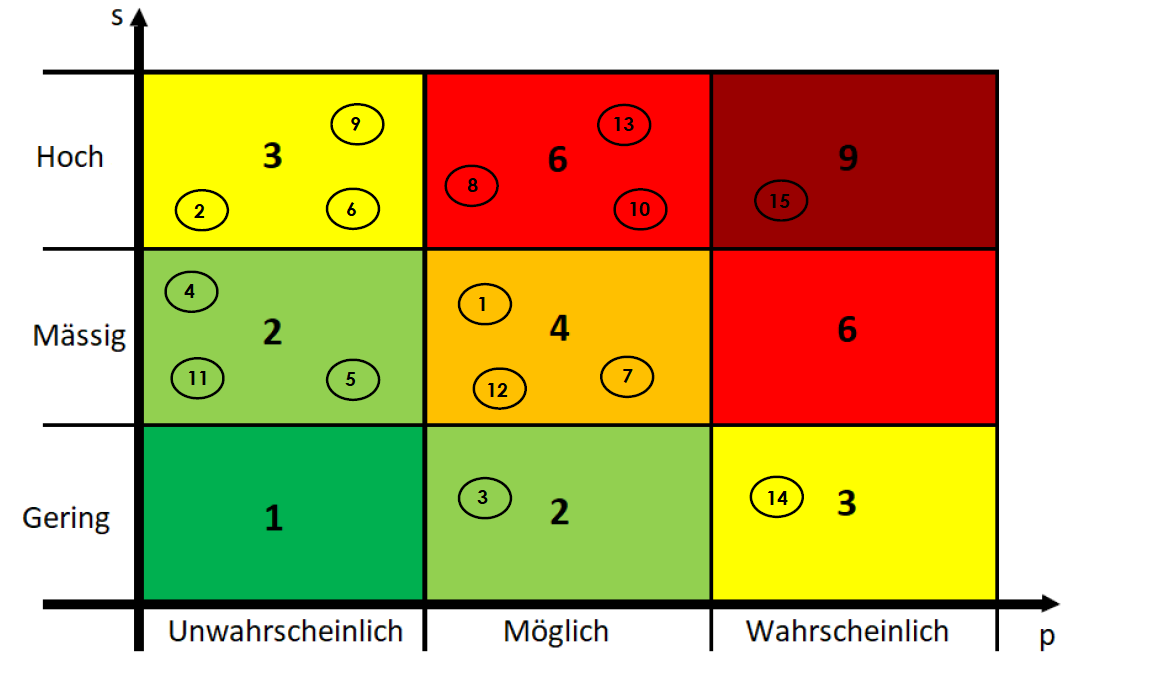
\includegraphics[width=13.5cm]{risiko1.png}
	\caption{Risikomatrix ohne Gegenmassnahmen}
\end{figure}

\newpage

Auf den Seiten 8 bis 10 werden die Risiken mittels Prävention dargestellt.
Ausserdem werden die Personen, die für die Prävention zuständig sind, aufgelistet.
Daraus folgt die Risikomatrix mittels Prävention:

\begin{figure}[htbp]
	\centering
	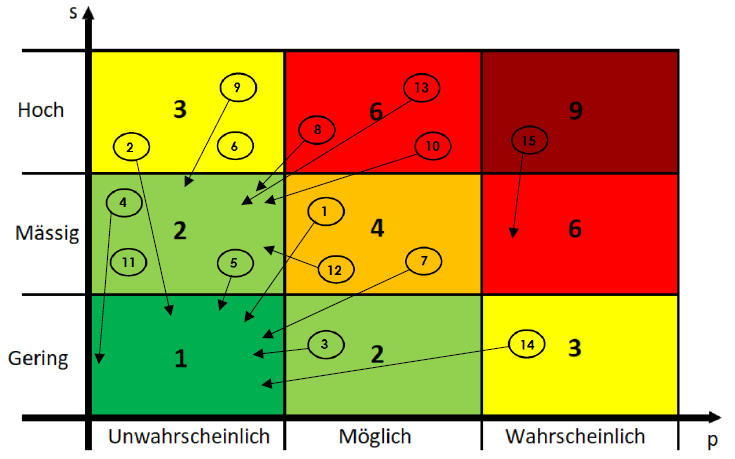
\includegraphics[width=13.5cm]{risiko2.png}
	\caption{Risikomatrix mit Gegenmassnahmen}
\end{figure}

Es gelten folgende Abkürzungen:

\begin{center}
\begin{tabular}{|c|c|}
	\hline
	\textbf{Kürzel} &  \textbf{Bedeutung} \\ \hline
	$S_{o}$ & Schadenausmass ohne Gegenmassnahmen \\ \hline
	$P_{o}$ & Eintrittswahrscheinlichkeit ohne Gegenmassnahmen \\ \hline
	$R_{o}$ & Risiko ohne Gegenmassnahmen \\ \hline
	$S_{m}$ & Schadenausmass mit Gegenmassnahmen \\ \hline
	$P_{m}$ & Eintrittswahrscheinlichkeit mit  Gegenmassnahmen \\ \hline
	$R_{m}$ & Risiko mit Gegenmassnahmen \\ \hline
\end{tabular}
\end{center}

\begin{landscape}

\begin{figure}[htbp]
	\centering
	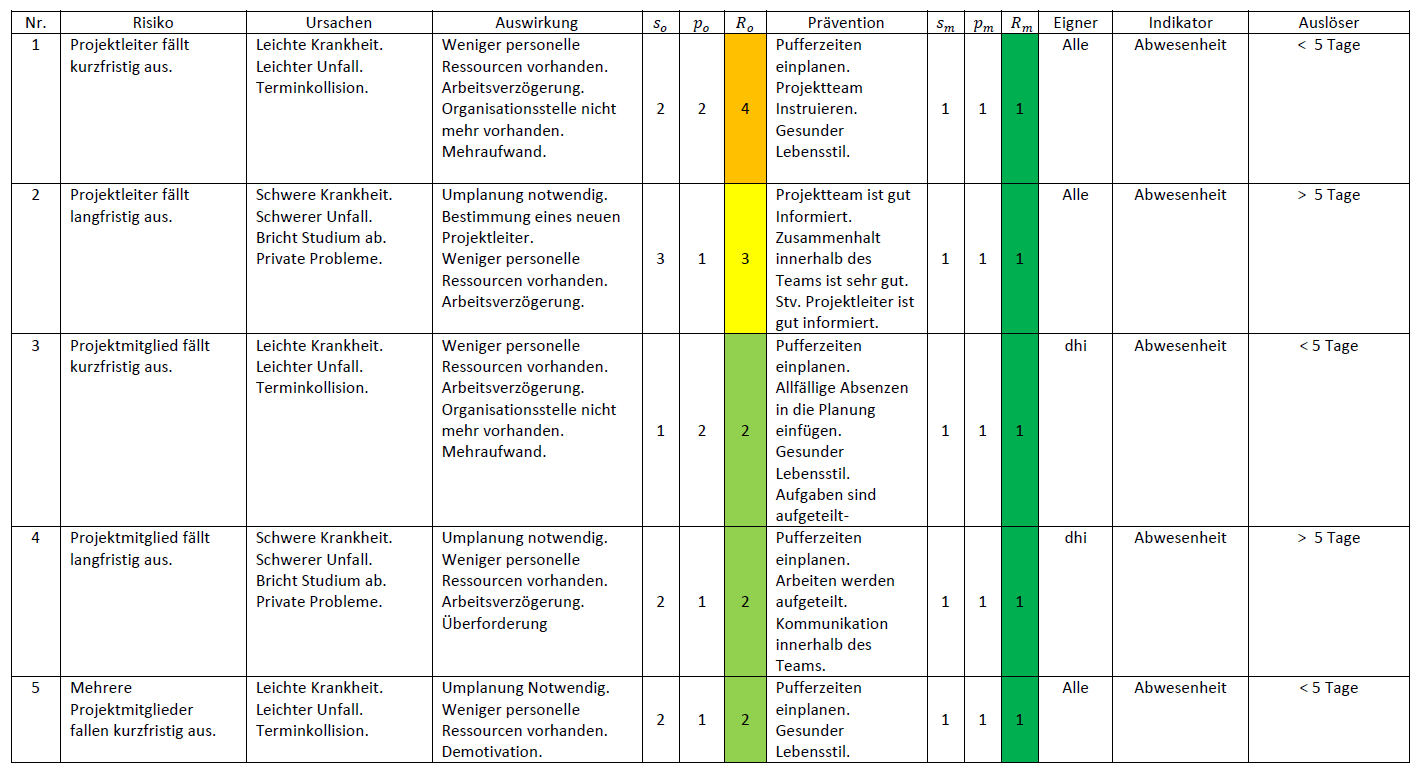
\includegraphics[width=25.5cm]{risikoAnalyse1.png}
\end{figure}

\begin{figure}[htbp]
	\centering
	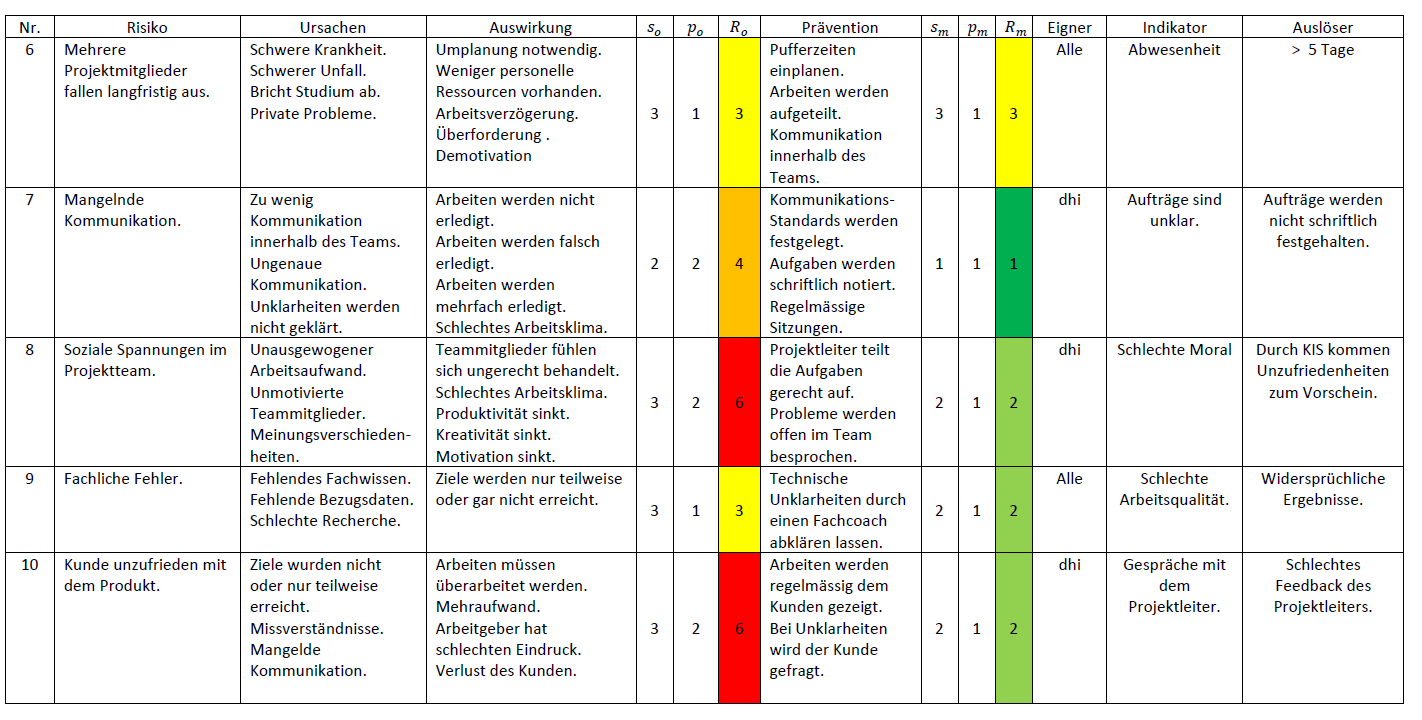
\includegraphics[width=25.5cm]{risikoAnalyse2.png}
\end{figure}

\begin{figure}[htbp]
	\centering
	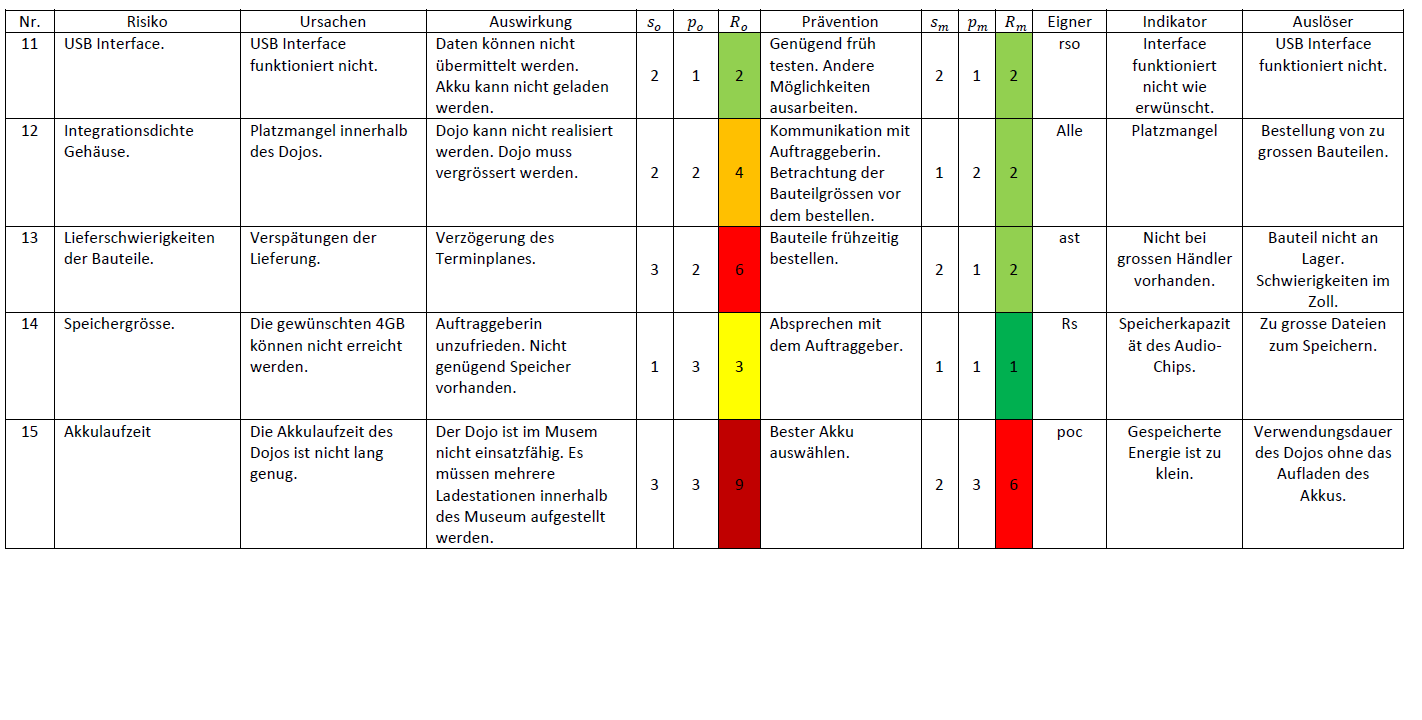
\includegraphics[width=25.5cm]{risikoAnalyse3.png}
\end{figure}

\end{landscape}

%%%%%%%%%%%%%%%%%%%%%%%%%%%%%%%%%%%%%%%%%%%%%%%%%%%%%%%%%%%%%%%%%%%%%%%%%%%%%%%%

\end{document}
